%\VignetteIndexEntry{sjemea}
%\VignetteKeywords{MEA}
%\VignettePackage{sjemea}
%\VignetteEngine{knitr::knitr}
\documentclass{article}\usepackage[]{graphicx}\usepackage[]{color}
%% maxwidth is the original width if it is less than linewidth
%% otherwise use linewidth (to make sure the graphics do not exceed the margin)
\makeatletter
\def\maxwidth{ %
  \ifdim\Gin@nat@width>\linewidth
    \linewidth
  \else
    \Gin@nat@width
  \fi
}
\makeatother

\definecolor{fgcolor}{rgb}{0.345, 0.345, 0.345}
\newcommand{\hlnum}[1]{\textcolor[rgb]{0.686,0.059,0.569}{#1}}%
\newcommand{\hlstr}[1]{\textcolor[rgb]{0.192,0.494,0.8}{#1}}%
\newcommand{\hlcom}[1]{\textcolor[rgb]{0.678,0.584,0.686}{\textit{#1}}}%
\newcommand{\hlopt}[1]{\textcolor[rgb]{0,0,0}{#1}}%
\newcommand{\hlstd}[1]{\textcolor[rgb]{0.345,0.345,0.345}{#1}}%
\newcommand{\hlkwa}[1]{\textcolor[rgb]{0.161,0.373,0.58}{\textbf{#1}}}%
\newcommand{\hlkwb}[1]{\textcolor[rgb]{0.69,0.353,0.396}{#1}}%
\newcommand{\hlkwc}[1]{\textcolor[rgb]{0.333,0.667,0.333}{#1}}%
\newcommand{\hlkwd}[1]{\textcolor[rgb]{0.737,0.353,0.396}{\textbf{#1}}}%

\usepackage{framed}
\makeatletter
\newenvironment{kframe}{%
 \def\at@end@of@kframe{}%
 \ifinner\ifhmode%
  \def\at@end@of@kframe{\end{minipage}}%
  \begin{minipage}{\columnwidth}%
 \fi\fi%
 \def\FrameCommand##1{\hskip\@totalleftmargin \hskip-\fboxsep
 \colorbox{shadecolor}{##1}\hskip-\fboxsep
     % There is no \\@totalrightmargin, so:
     \hskip-\linewidth \hskip-\@totalleftmargin \hskip\columnwidth}%
 \MakeFramed {\advance\hsize-\width
   \@totalleftmargin\z@ \linewidth\hsize
   \@setminipage}}%
 {\par\unskip\endMakeFramed%
 \at@end@of@kframe}
\makeatother

\definecolor{shadecolor}{rgb}{.97, .97, .97}
\definecolor{messagecolor}{rgb}{0, 0, 0}
\definecolor{warningcolor}{rgb}{1, 0, 1}
\definecolor{errorcolor}{rgb}{1, 0, 0}
\newenvironment{knitrout}{}{} % an empty environment to be redefined in TeX

\usepackage{alltt}
\usepackage{mathpazo}
\renewcommand{\sfdefault}{lmss}
\renewcommand{\ttdefault}{lmtt}
\usepackage[T1]{fontenc}
\usepackage[a4paper,left=2cm,right=4cm,top=2cm,bottom=2cm]{geometry}
\usepackage{setspace}
\usepackage{listings}
\usepackage{verbatim}

\usepackage{xspace,amsmath}
\newcommand{\um}{\ensuremath{\mu \text{m}}\xspace}
\usepackage{url}
\usepackage[authoryear]{natbib}
\newcommand{\dynamic}{(Dynamic)}
\newcommand{\static}{(Static)}
\newcommand{\hdfgroup}[1]{\texttt{#1}}
%% Place all figures at end of paper?
%%\usepackage[noheads,nomarkers]{endfloat}
\IfFileExists{upquote.sty}{\usepackage{upquote}}{}

\begin{document}

\onehalfspacing
\title{meadq package: From A to Z }

\author{Diana Hall}
\date{\today}

\maketitle


\section*{Installation}
To install this package, and then view this introductory vignette, do:

\begin{knitrout}
\definecolor{shadecolor}{rgb}{0.969, 0.969, 0.969}\color{fgcolor}\begin{kframe}
\begin{alltt}
\hlstd{tarfile.path} \hlkwb{=} \hlstr{"F:/R/Rpackage_meadq/meadq_1.0.1.tar.gz"}
\hlkwd{install.packages}\hlstd{(}\hlkwc{pkgs} \hlstd{= tarfile.path,} \hlkwc{type} \hlstd{=} \hlstr{"source"}\hlstd{,} \hlkwc{repos} \hlstd{=} \hlkwa{NULL}\hlstd{)}
\hlkwd{vignette}\hlstd{(}\hlstr{"meadq-intro"}\hlstd{,} \hlkwc{package} \hlstd{=} \hlstr{"meadq"}\hlstd{)}
\end{alltt}
\end{kframe}
\end{knitrout}


Alternatively, if you want to get the latest version of the package,
you can install it in the following manner:
\begin{knitrout}
\definecolor{shadecolor}{rgb}{0.969, 0.969, 0.969}\color{fgcolor}\begin{kframe}
\begin{alltt}
\hlkwd{install.package}\hlstd{(}\hlstr{"devtools"}\hlstd{)}  \hlcom{# note: need R v.>=3.1.0}
\hlcom{# to install devtools, use CRAN}
\hlkwd{require}\hlstd{(devtools)}
\hlkwd{install_github}\hlstd{(}\hlstr{"dianaransomhall/meadq"}\hlstd{)}
\end{alltt}
\end{kframe}
\end{knitrout}

You can browse the package sources via the URL
\url{http://github.com/dianaransomhall/meadq}.


\section*{Setup}
This file is a vignette, written in R, as a reproducible research
document.

\begin{knitrout}
\definecolor{shadecolor}{rgb}{0.969, 0.969, 0.969}\color{fgcolor}\begin{kframe}
\begin{alltt}
\hlkwd{require}\hlstd{(meadq)}
\end{alltt}


{\ttfamily\noindent\color{warningcolor}{\#\# Warning: there is no package called 'meadq'}}\begin{alltt}
\hlkwd{require}\hlstd{(knitr)}
\hlstd{opts_chunk}\hlopt{$}\hlkwd{set}\hlstd{(}\hlkwc{cache} \hlstd{=} \hlnum{TRUE}\hlstd{)}
\hlstd{opts_chunk}\hlopt{$}\hlkwd{set}\hlstd{(}\hlkwc{dev} \hlstd{=} \hlstr{"pdf"}\hlstd{)}
\end{alltt}
\end{kframe}
\end{knitrout}


\section*{Introduction}

This is a short introduction to the abilities of the meadq package
for analysis of multielectrode array data.  It is not a comprehensive
guide, but simply gives examples of what can be done with the package.
The package contains some example data sets which are used here to
demonstrate various routines.  

\subsection*{Help pages}
A list of help pages associated with the package is given by
\verb+help(package='meadq')+ command:
\begin{knitrout}
\definecolor{shadecolor}{rgb}{0.969, 0.969, 0.969}\color{fgcolor}\begin{kframe}


{\ttfamily\noindent\bfseries\color{errorcolor}{\#\# Error: there is no package called 'meadq'}}\end{kframe}
\end{knitrout}



\section*{creating .h5 Files from text files of spike trains}

Convert the recorded data, which may be in a proprietary or otherwise non universal file type, into a type which may be read in by various softwares.  Following suggestions from the "program on Standards for Datasharing" by the International neuroinformatics coordinating facility \url{datasharing.incf.ord/ep/HDF5_data_standard}, code is provided to convert axion alpha map files to .h5 files that link spike train to meta-data about the experiment.  Current functionality is restricted to experimental meta data limited to a handful of variabes. However, additional information may be built in by creating a new function. 

\begin{knitrout}
\definecolor{shadecolor}{rgb}{0.969, 0.969, 0.969}\color{fgcolor}\begin{kframe}
\begin{alltt}
\hlcom{# For example, choose .mapTimestamps:}
\hlkwd{print}\hlstd{(}\hlkwd{system.file}\hlstd{(}\hlstr{"extdata"}\hlstd{,} \hlstr{"ON_20140205_MW1007-26_DIV07_001.mapTimestamps"}\hlstd{,}
    \hlkwc{package} \hlstd{=} \hlstr{"meadq"}\hlstd{))}
\end{alltt}
\begin{verbatim}
## [1] ""
\end{verbatim}
\begin{alltt}
\hlkwd{make.axion.map.to.h5.dh}\hlstd{()}
\end{alltt}


{\ttfamily\noindent\bfseries\color{errorcolor}{\#\# Error: could not find function "{}make.axion.map.to.h5.dh"{}}}\end{kframe}
\end{knitrout}


\subsection{What is the ``s[[i]]'' object?}

A convention of the program is that all data referring to a recording
is stored within an object of class \texttt{mm.s}, which is actually a
list.  So, when new data/results are collected for a recording, I tend
to add the new information into that object (e.g. see how burst
analysis results are stored).

The most important items in the list are:
\begin{description}
\item[NCells] The number of units in the recording.
\item[rec.time] The start and end time of the recording.
\item[spikes] A list of vectors.  Element $i$ of the list is the
  vector of spike trains for unit $i$.  Each spike train is ordered, smallest first.
\item[nspikes] A vector.  $nspikes[i]$ is the number of spikes in
  train i.
\item[layout] Information regarding the spatial layout of the units.
\end{description}

\section*{Burst analysis}

Burst identification is done with:
\begin{enumerate}
\item Max Interval method, as described by Neuroexplorer \citep{neuroexplorer}

\end{enumerate}

The MaxInterval method.
\begin{knitrout}
\definecolor{shadecolor}{rgb}{0.969, 0.969, 0.969}\color{fgcolor}\begin{kframe}
\begin{alltt}
\hlstd{data.file} \hlkwb{<-} \hlkwd{system.file}\hlstd{(}\hlstr{"data"}\hlstd{,} \hlstr{"example_ont_data.rda"}\hlstd{,} \hlkwc{package} \hlstd{=} \hlstr{"meadq"}\hlstd{)}
\hlkwd{load}\hlstd{(data.file)}
\end{alltt}


{\ttfamily\noindent\color{warningcolor}{\#\# Warning: cannot open compressed file '', probable reason 'Invalid argument'}}

{\ttfamily\noindent\bfseries\color{errorcolor}{\#\# Error: cannot open the connection}}\end{kframe}
\end{knitrout}


So, for example, for electrode 2, we see the following bursts (just
taking the head as there are many of them.  We can also easily plot
the number of bursts on each electrode.

\begin{knitrout}
\definecolor{shadecolor}{rgb}{0.969, 0.969, 0.969}\color{fgcolor}\begin{kframe}
\begin{alltt}
\hlcom{# head(s[[3]]$allb[[2]]) nbursts <- sapply(s[[3]]$allb, nrow) plot(nbursts,}
\hlcom{# xlab='Electrode number', ylab='Number of bursts', bty='n', las=1)}
\end{alltt}
\end{kframe}
\end{knitrout}



Once bursts are computed the resulting burst information can be
visualized on a raster assuming that the burst information is stored
in the \verb+s$allb+ component of the object.  Here we ask to see the
burst information for twenty seconds of data from just the first five trains.

\begin{knitrout}
\definecolor{shadecolor}{rgb}{0.969, 0.969, 0.969}\color{fgcolor}\begin{kframe}
\begin{alltt}
\hlcom{# plot(s[[3]], beg=100, end=200, show.bursts=TRUE, whichcells=1:5)}
\end{alltt}
\end{kframe}
\end{knitrout}


Bursts are indicated with a red horizontal line, and the blue number
indicates the number of spikes in the burst.


Note: a Hidden-Markov Model (HMM) for burst analysis in R \citep{Tokdar2010}
is available in the following package:
\url{http://www.stat.duke.edu/~st118/Software/}.

can be used within this package, but in principle (computation time
aside as I expect an HMM to be slow) there should be no issue.  There
is also a generic ``bursts'' package:
\url{http://cran.r-project.org/web/packages/bursts/bursts.pdf}.



\section*{Network spikes}

Network spikes are periodic elevations in activity across the whole
array \citep{Eytan2006}.  The following example shows how they are computed.
In the resulting graph, the population ``firing rate'' (the number of
active electrodes here) is shown on the y axis, time (in seconds) on
the x axis.  The horizontal red line is a threshold set for the
minimum number of active electrodes to determine a ``network spike''.
The blue dots are the peak of each network spikes.

The mean network spike is also shown, averaged across all the network
spikes in the recording.

\begin{knitrout}
\definecolor{shadecolor}{rgb}{0.969, 0.969, 0.969}\color{fgcolor}\begin{kframe}
\begin{alltt}
\hlkwd{example}\hlstd{(compute.ns,} \hlkwc{package} \hlstd{=} \hlstr{"sjemea"}\hlstd{)}
\end{alltt}
\begin{verbatim}
## 
## cmpt.n> data.file <- system.file("examples", "TC89_DIV15_A.nexTimestamps",
## cmpt.n+                          package = "sjemea")
## 
## cmpt.n> s <- sanger.read.spikes( data.file, beg=400, end=700)
## 
## cmpt.n> s$ns <- compute.ns(s, ns.T=0.003, ns.N=10,sur=100)
## 
## cmpt.n> plot(s$ns, ylab='Count', xlab='Time (s)')
\end{verbatim}
\end{kframe}
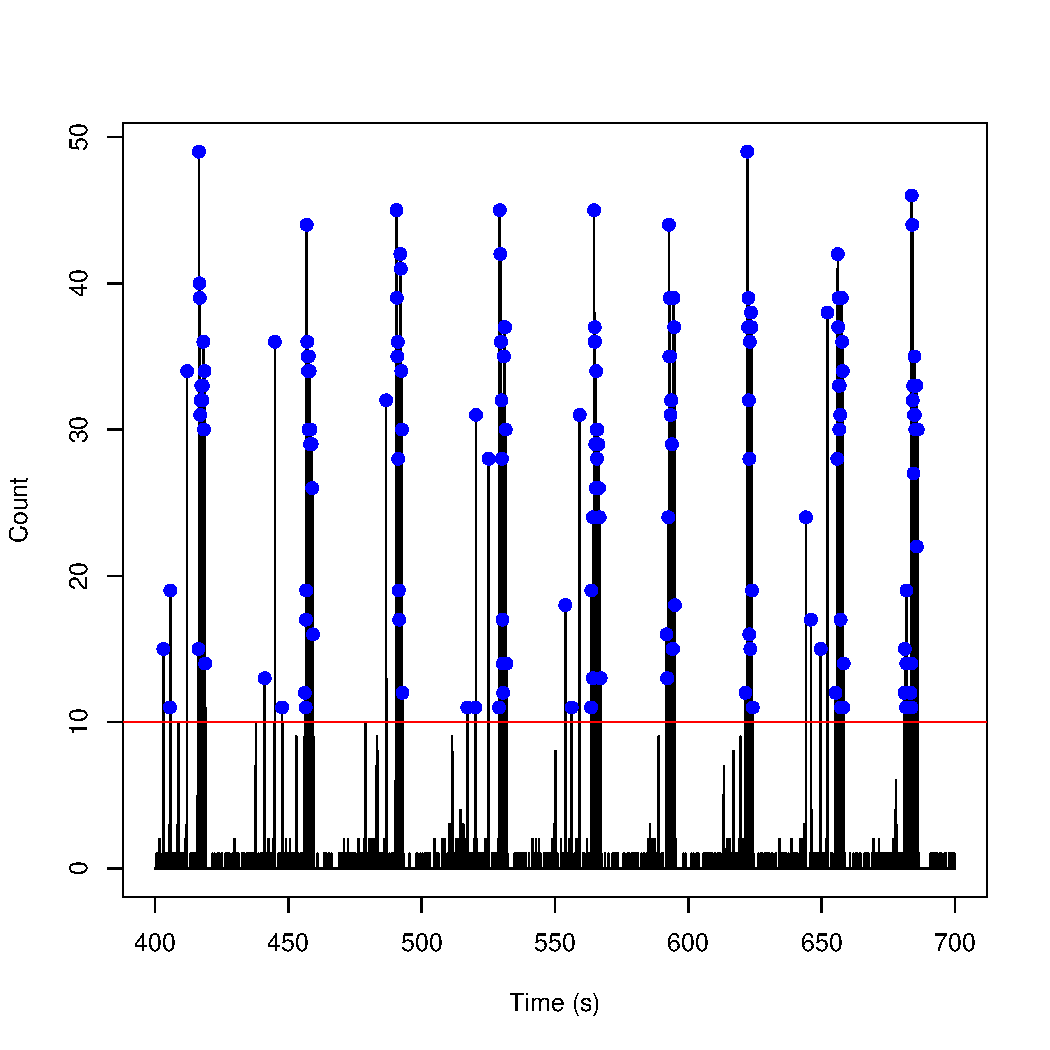
\includegraphics[width=\maxwidth]{figure/unnamed-chunk-21} 
\begin{kframe}\begin{verbatim}
## 
## cmpt.n> plot(s$ns, xlim=c(450, 500),
## cmpt.n+      xlab='Time (s)', ylab='Count')
\end{verbatim}
\end{kframe}
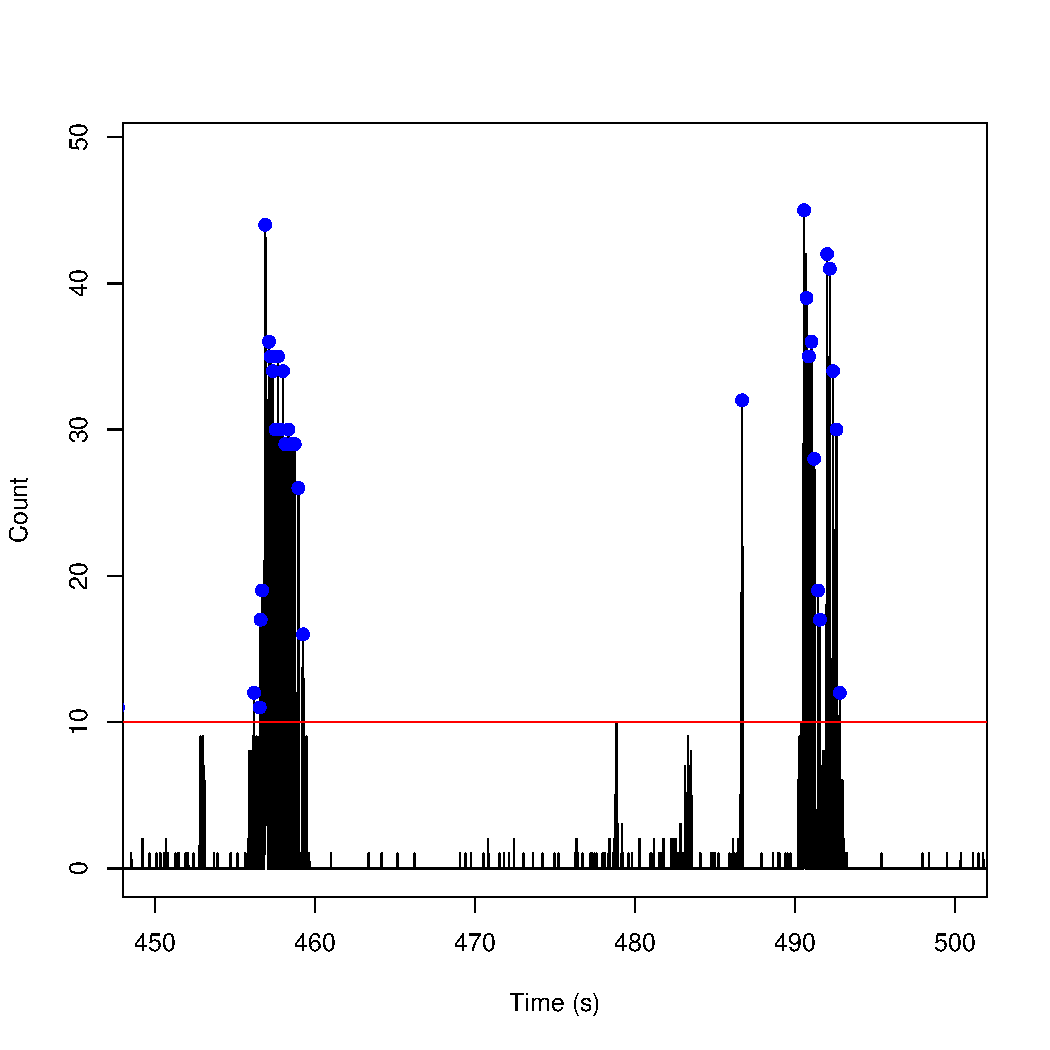
\includegraphics[width=\maxwidth]{figure/unnamed-chunk-22} 
\begin{kframe}\begin{verbatim}
## 
## cmpt.n> plot(s$ns$mean, xlab='Time (s)', ylab='Count', main='Mean NS')
\end{verbatim}
\end{kframe}
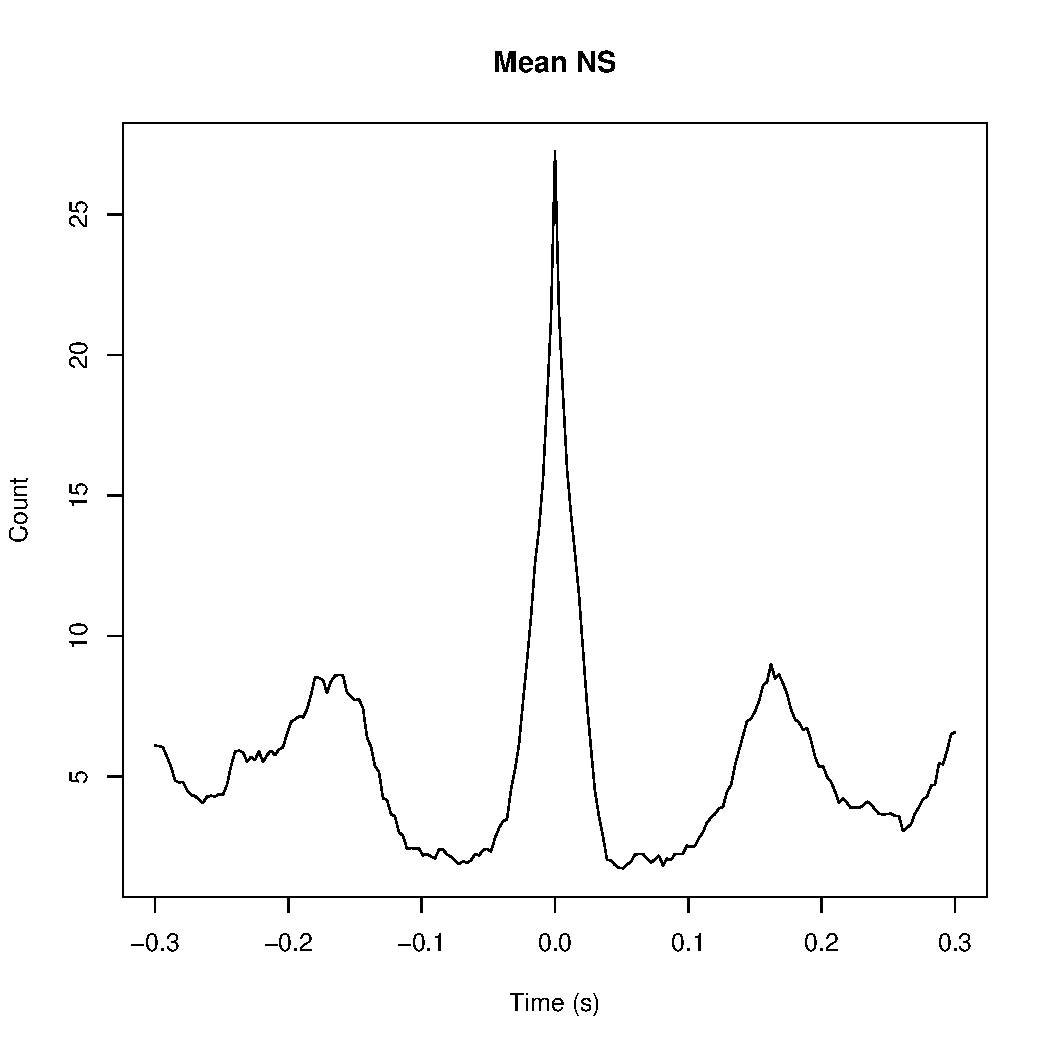
\includegraphics[width=\maxwidth]{figure/unnamed-chunk-23} 
\begin{kframe}\begin{verbatim}
## 
## cmpt.n> summary(s$ns)
## 167 network spikes
## recruitment 27.23 +/- 10.52
## FWHM 0.023 +/- 0.013 (s)
## 
## cmpt.n> s$ns$brief
##         n    peak.m   peak.sd    durn.m   durn.sd 
## 167.00000  27.23353  10.51559   0.02315   0.01264 
## 
## cmpt.n> ## show.ns(s$ns)  # This shows each network spike!  Can take a long time.
## cmpt.n> 
## cmpt.n> 
## cmpt.n>
\end{verbatim}
\end{kframe}
\end{knitrout}


\bibliographystyle{jneurosci}
\bibliography{sjemea}

\subsection*{Compiling this document}

\begin{knitrout}
\definecolor{shadecolor}{rgb}{0.969, 0.969, 0.969}\color{fgcolor}\begin{kframe}
\begin{alltt}
\hlkwd{require}\hlstd{(knitr)}
\hlkwd{knit2pdf}\hlstd{(}\hlstr{"meadq-into.Rnw"}\hlstd{)}
\end{alltt}
\end{kframe}
\end{knitrout}





\end{document}
